\section{Analiza tematu}
Celem niniejszej pracy jest zobrazowanie zależności w przesyłach danych, między poszczególnymi stacjami działającymi w sieci opartej o protokół Master - Slave.

\section{Budowa i działanie sieci Master - Slave}
W sieciach opartych o model komunikacyjny Master - Slave, można wyróżnić wiele stacji typu slave, oraz jedną stację master. Jedynie stacja master może swobodnie wysyłać i żądać dane od innych stacji. Slave natomiast jeśli potrzebuje jakiejś informacji, której cykliczna transmisja nie została przewidziana na etapie projektowania sieci musi skorzystać z tzw. wymiany wyzwalanej (na które dodatkowo należy wziąć poprawkę przy projektowaniu scenariusza wymian w sieci).
	\begin{figure}[h]
		\centering
		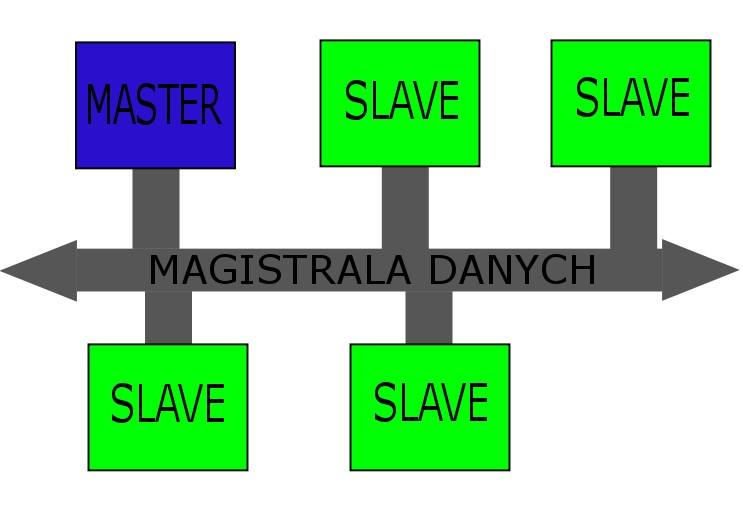
\includegraphics[width=0.7\textwidth]{./img/siec.jpg}
		\caption{Struktura sieci master-slave}
		\label{fig:siec}
	\end{figure}

	\subsection{Scenariusz wymian}
	Ze względu na swój sposób działania sieć master - slave daje nam ogromny zakres kontroli nad wymianami danych zachodzącymi w sieci. Jest tak, ponieważ każdą z nich trzeba samemu zaplanować - robi się to za pomocą tzw. \textit{scenariusza wymian}, projektowanego równolegle z siecią i zależnemu od pracy poszczególnych komponentów systemu rozproszonego.\\
	W scenariuszu znaleźć się muszą wszystkie wymiany, których dokonanie w określonym okresie czasu jest niezbędne dla poprawnego działania systemu (oraz spełniania przez niego wymagań czasowych).\\
	Przyjmuje on postać tabeli, w której zapisane są takie parametry jak :
	\begin{itemize}
		\item tryb transmisji danych
		\begin{itemize}
			\item ASCII
			\item RTU
		\end{itemize}
		\item liczba bitów stopu i parzystości
		\item liczba bitów przypadająca na jeden znak transmisji
		\item prędkość transmisji
	\end{itemize}
	Dodatkowo uwzględniane są parametry indywidualne dla każdej wymiany:
	\begin{itemize}
		\item numer wymiany
		\item adres abonenta
		\item kod operacji
		\item adres danych jednostki master do wysłania, bądź adres danych do otrzymania od stacji slave
		\item rozmiar danych
		\item wybór trybu - wymiana periodyczna bądź wyzwalana
		\item ustalenie czy należy automatycznie usunąć abonenta przy braku odpowiedzi
		\item adres słowa raportu wymiany
		\item parametry związane raczej ze sprzętową konfiguracją wymiany:
		\begin{itemize}
			\item graniczny czas oczekiwania na odpowiedź $ T_{OODP} $
			\item ilość prób ponownego połączenia w przypadku przekroczenia czasu $ T_{OODP} $, określane dalej jako $ L_{REP} $
			\item liczba cykli sieci, po których podjęta zostanie ponownie próba komunikacji (w przypadku gdy żadna z prób komunikacji z punktu powyższego nie zakończyła się sukcesem), określana dalej jako $ L_{COCZK} $
			\item długość przerwy między kolejnymi transmisjami rozgłoszeniowymi
			\item czas opóźnienia przed transmisją ramki oraz po jej zakończeniu.
			\item czas autoryzacji mający znaczenie przy pracy z modemami
		\end{itemize}
	\end{itemize}
	Jako, że nie każde dane należy transmitować w regularnych odstępach czasu, dodany został mechanizm tzw. \textit{wymian wyzwalanych}. Jest to wymiana, którą może zainicjować stacja slave w pakiecie odpowiedzi - informuje ona stację slave, że potrzebuje określone dane, a master z czasem je jej dostarczy.\\
	\\
	Warto pamiętać, że zawartość scenariusza wymian, oraz sposób konfiguracji go będzie się różnić w zależności od użytego koprocesora sieci, oraz wybranego protokołu.